%--------------------------------------------------------------------
\medskip
\section{Roles Tácticos}
La implementación de los roles tácticos la hemos realizado a través de la interfaz \texttt{TacticalRole} que contiene dos métodos importantes:
\begin{itemize}
 \item Método \texttt{initialize()}. Este método realiza la inicialización de la estructura táctica que se va a utilizar. Por ejemplo, en el caso de que un rol se implemente con una máquina de estados, pues crear e inicializar dicha máquina.
 \item Método \texttt{update()}. Este método realiza la actualización de la estructura táctica inicializada y las acciones pertinentes dependiendo de dicha actualización.
\end{itemize}

Ambos métodos reciben como parámetro el personaje al que se va a aplicar los comportamientos obtenidos tras la inicialización/actualización de la estructura táctica. \\

También contiene los siguientes métodos:
\begin{itemize}
 \item \texttt{getVelocityFactor()}. Devuelve el factor de velocidad que un rol tiene para un determinado terreno. Este método devolverá un valor entre 0 y 1 que se usa para modificar la velocidad que se aplica a un personaje antes de aplicar un determinado steering. Con este método, se permite que los personajes, dependiendo de su rol, vayan a una velocidad dependiendo del terreno por el que vayan.
 \item \texttt{getTacticalCost()}. Devuelve el coste táctico que un rol tiene asociado a un determinado terreno. 
 \item \texttt{getMaxDistanceOfAttack()}. Devuelve la máxima distancia de ataque de un rol.
 \item \texttt{getDamageToDone()}. Devuelve el daño que puede hacer al atacar un rol.
 \item \texttt{getMaxSpeed()}. Devuelve la máxima velocidad a la que puede ir un rol.
\end{itemize}

Los roles tácticos que hemos implementado nosotros han sido: soldado y arquero, tanto ofensivos como defensivos. Tanto los ofensivos como los defensivos, tienen los mismos valores para los métodos anteriores (dependiendo de si son arqueros o soldados). La diferencia entre ellos está en la estructura con la que se han implementado: los roles ofensivos (tanto soldados como arqueros) se han implementado con un árbol de decisión; mientras que los roles defensivos (tanto soldados como arqueros) se han implementado con una máquina de estados. En la siguientes subseciones, se comentará más en profundidad sobre cada uno de estos roles. \\

Todo esto se encuentra dentro del paquete \texttt{com.mygdx.iadevproject.aiTactical.roles} del proyecto.


%--------------------------------------------------------------------
\medskip
\subsection{Roles defensivos}
Ambos roles defensivos (arquero y soldado) se han implementado como una máquina de estados. Para ello, se ha hecho uso de la interfaz \texttt{StateMachine} proporcionada por la librería LibGDX \cite{stateMachine}. Esta máquina de estados hace uso de la interfaz \texttt{State} proporcionada también por la librería LibGDX, que proporciona los siguientes métodos:
\begin{itemize}
  \item \texttt{enter()} que se llama cada vez que se entra al estado. 
  \item \texttt{update()} que se llama cada vez que la máquina de estados se actualiza y este es el estado actual de la máquina.
  \item \texttt{exit()} que se llama cuando se sale del estado.
  \item \texttt{onMessage()} que se llama si la entidad recibe un mensaje del despachador de mensajes mientras está en este estado. 
\end{itemize}

Estos métodos reciben como parámetro una entidad con la que se puede trabajar en cada método. En nuestro caso, esta entidad será un objeto de la clase \texttt{Character}. \\

La interfaz \texttt{StateMachine} proporciona varios métodos para poder realizar distintas acciones con la máquina de estados. De entre ellos, las que hemos utilizado son:
\begin{itemize}
 \item \texttt{setInitialState()}. Se emplea para establecer el estado inicial de la máquina, que se le pasa como parámetro.
 \item \texttt{isInState()}. Comprueba si la máquina está en el estado pasado como parámetro.
 \item \texttt{changeState()}. Cambia el estado actual al estado pasado como parámetro.
 \item \texttt{update()}. Actualiza la máquina: esto implica llamar al método \texttt{update()} del estado actual. 
\end{itemize}

Al crear la máquina de estados, esta pide que se indique el objeto ``propietario'' de la máquina de estados; esto es, el objeto que la máquina pasa como parámetro en los métodos de la interfaz \texttt{State}. Para introducirle los estados que nosotros queremos a la máquina de estados, hemos tenido que crear clases concretas que implementaran la interfaz \texttt{State} anteriormente mencionada. Para todos los estados, la entidad que recibe como parámetro es de la clase \texttt{Character}. \\

Por último, en las Figuras \ref{defensivos:soldado} y \ref{defensivos:arquero} se muestran las máquinas de estados concretas para los soldados y arqueros defensivos. La idea que hay detrás de estos roles es que ambos tienen que patrullar una zona (los soldados patrullan su base, los arqueros patrullan los waypoints de los puentes), hasta que se encuentran a un enemigo cerca y lo atacan, siempre y cuando no estén lejos de su base/waypoint. Como se trata de un rol defensivo, estos van a estar atacando hasta que se mueran. Por último, debido a que hay 6 waypoints para cada patrullar, si hay más arqueros defensivos que waypoints, estos se quedarán a la espera (haciendo cosas aleatorias) de que uno se libere para cogerlo.
\begin{figure}[!th]
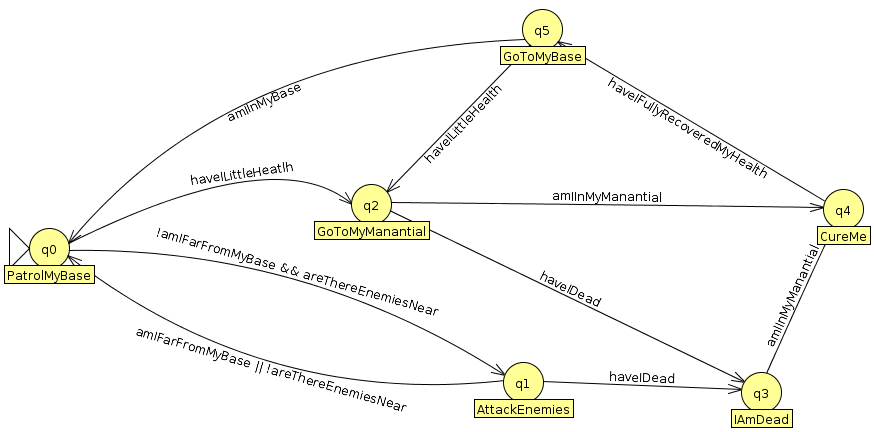
\includegraphics[scale=0.6]{defensive-soldier}
\centering
\caption{Máquina de estados para el soldado defensivo.}
\label{defensivos:soldado}
\end{figure}
\begin{figure}[!th]
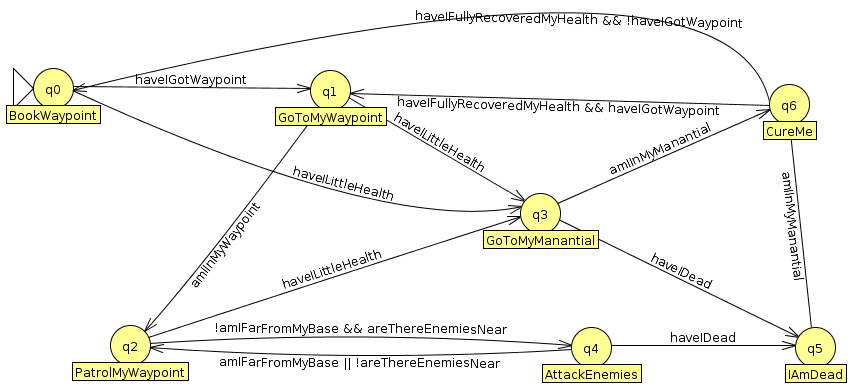
\includegraphics[scale=0.6]{defensive-archer}
\centering
\caption{Máquina de estados para el arquero defensivo.}
\label{defensivos:arquero}
\end{figure}

Es importante destacar los siguientes puntos:
\begin{itemize}
 \item Si no se cumplen las condiciones necesarias en el estado actual, no se cambia de estado. De ahí que no haya transiciones en las figuras sobre los propios estados. Cuando no se cambia de estado, exceptuando el estado \texttt{AttackEnemies} y los que requieren el uso del Pathfinding, la máquina de estados no se actualiza, ya que cuando se entró al estado, se calcularon los comportamientos correspondientes y el personaje sigue haciendo lo mismo, por lo que no es necesario calcularlo de nuevo.
 
 \item Los estados que requieran el uso del Pathfinding (\texttt{GoToMyBase, GoToMyManantial y GoToMyWaypoint}) para evitar que se esté calculando el Pathfinding cada vez que se actualice el estado, hacemos uso del método \texttt{enter()} del estado para que cada vez que se entre se calcule el Pathfinding, mientras que en el método \texttt{update()} lo que se hace es aplicar el Pathfinding para que nos dé el siguiente punto a seguir.
 
 \item En el estado \texttt{AttackEnemies} se ataca siempre al enemigo más cercano (de ahí que se tenga que actualizar el estado si no hemos cambiado). También el personaje intenta alejarse del objetivo a una distancia en la que él pueda atacar. Así pues permitimos que aquellos personajes que tengan una distancia de ataque mayor (los arqueros en nuestro caso), puedan sacar provecho de ello cuando se ataca. También se mira al personaje que se ataca.
 
 \item En el estado \texttt{IAmDead} se traslada directamente el personaje a la posición de su manantial, estableciendo su posición a la posición del manantial.
 
 \item En el estado \texttt{BookWaypoint} mientras que espera a tener un waypoint libre, el personaje lo que hace es moverse de manera aleatoria (aplicando un Wander), para evitar que se quede parado.
 
 \item Debido a que los arqueros defensivos tienen que reservar el waypoint que tienen que patrullar, solamente se va a liberar un waypoint cuando el arquero que lo está patrullando muere. Es decir, entrar al estado \texttt{IAmDead} implica que el arquero deja libre su waypoint para que otro pueda cogerlo. Sin embargo, cuando un arquero entra al estado \texttt{GoToMyManantial} porque quiere curarse, no se libera el waypoint porque no ha muerto. 
 
 \item Consideramos que de primeras, los soldados se encuentran en la base (o cerca de ella), por lo que en su estado inicial no se hace ningún Pathfinding. En cambio, como los arqueros, mientras que no tienen un waypoint que patrullar, se mueven de manera aleatoria, cuando reserva un waypoint, sí se calcula un Pathfinding para ir a él, porque puede estar en la otra punta del mapa.
\end{itemize}


%--------------------------------------------------------------------
\medskip
\subsection{Roles ofensivos}
